%%%%%%%%%%%%%%%%%%%%%%%%%%%%%%%%%%%%%%%%%%%%%%%%%%%%%%%%%%%%%%%%%%%%%%%%%%%%%%%%
% Chapter 2: Conceptos
%%%%%%%%%%%%%%%%%%%%%%%%%%%%%%%%%%%%%%%%%%%%%%%%%%%%%%%%%%%%%%%%%%%%%%%%%%%%%%%%

%+++++++++++++++++++++++++++++++++++++++++++++++++++++++++++++++++++++++++++++++
En este capítulo se abordarán todos aquellos conceptos teóricos que han surgido
a lo largo del proyecto y son necesarios para entender correctamente la línea
del trabajo.


%+++++++++++++++++++++++++++++++++++++++++++++++++++++++++++++++++++++++++++++++
\section{Visión artificial}
\label{2:sec:1}
% https://campusvirtual.ull.es/1516/course/view.php?id=202
% https://es.wikipedia.org/wiki/Visi%C3%B3n_artificial
% https://en.wikipedia.org/wiki/Computer_vision
% J. GONZÁLEZ JIMÉNEZ, "Visión Por Computador", Editorial Paraninfo. 2000

La visión artificial por computador, es la disciplina científica que se basa en
la adquisición, procesamiento y análisis de las imágenes que se toman del mundo
real, con el objetivo de obtener información relevante acerca de ellas:
detección de objetos, seguimiento del movimiento, reconocimiento de eventos,
etc. Un ejemplo que podemos ver en nuestro día a día, es la detección de caras
en una escena capturada por una cámara digital o smartphone, mediante el uso de
téncicas de reconocimiento de patrones.

Al igual que sucede en otras áreas de la inteligencia artificial, la visión
artificial tiene como objetivo principal obtener la información explícita y el
significado de la realidad de la misma manera que lo haría un ser biológico.

El avance progresivo del hardware con nuevos procesadores digitales de señales
(DSP) y unidades de procesamiento gráfico (GPU), junto con nuevas tecnologías y planteamientos de cómputo como la computación paralela, ha permitido que en los
últimos años se haya podido implementar nuevos algortimos más rápidos y
eficientes, necesarios para ser utilizados en ámbitos críticos, como sistemas
en tiempo real.

%--------------------------------------
\subsection{Objetivos}

\textcolor{red}{Lorem ipsum dolor sit amet, consectetur adipisicing elit, sed do
 eiusmod tempor incididunt ut labore et dolore magna aliqua. Ut enim ad minim 
 veniam, quis nostrud exercitation ullamco laboris nisi ut aliquip ex ea commodo 
 consequat. Duis aute irure dolor in reprehenderit in voluptate velit esse cillum
 dolore eu fugiat nulla pariatur. Excepteur sint occaecat cupidatat non proident,
 sunt in culpa qui officia deserunt mollit anim id est laborum.}

\textcolor{red}{Lorem ipsum dolor sit amet, consectetur adipisicing elit, sed do
 eiusmod tempor incididunt ut labore et dolore magna aliqua. Ut enim ad minim 
 veniam, quis nostrud exercitation ullamco laboris nisi ut aliquip ex ea commodo 
 consequat. Duis aute irure dolor in reprehenderit in voluptate velit esse cillum
 dolore eu fugiat nulla pariatur. Excepteur sint occaecat cupidatat non proident,
 sunt in culpa qui officia deserunt mollit anim id est laborum.}

%--------------------------------------
\subsection{Dificultades}
La capacidad visual es uno pilares de la inteligencia humana. Su implementación
en la rotótica supone también un importante avance en la inteligencia artificial.
Sin embargo, mientras que la percepción visual es algo innato y cotidiano para
nosotros, la visión artificial es muy compleja y conlleva muchas dificultades.
Entre las principales dificultades, destacan:

\begin{itemize}
  \item \textbf{Mundo tridimensional:} mientras que las imágenes que se obtienen
  con una cámara son bidimensionales, el mundo que nos rodea no. Es necesario 
  realizar las transformaciones correspondientes para obtener valores correctos.
  \item \textbf{Zonas de interés:} se necesita extraer elementos de información 
  sutiles en imágenes complejas, por lo que entre tanta información es necesario
  reconocer formas, colores, etc.
  \item \textbf{Carácter dinámico de las escenas:} el mundo está vivo, por lo
  que en las imágenes que se toman muchos elementos están en movimiento. Por 
  otro lado, otros factores como luminosidad, contraste, foco... pueden marcar
  una importante diferencia, y por desgracia, estos factores son variables, no
  se pueden controlar.
\end{itemize}

%--------------------------------------
% \subsection{Reconocimiento}

% Detección de objetos

%--------------------------------------
% \subsection{Motion Analysis}

% Video grabación de imágenes de seguridad

%--------------------------------------
% \subsection{Reconstrucción}


%+++++++++++++++++++++++++++++++++++++++++++++++++++++++++++++++++++++++++++++++
\section{Visión estéreo}
\label{2:sec:2}
% http://vision.deis.unibo.it/~smatt/Seminars/StereoVision.pdf
% http://www.cesfelipesegundo.com/revista/articulos2011/Guerrero,%20J.M.pdf

La visión estereoscópica o visión estéreo, es la técnica capaz de extraer
información tridimensional (profundidad) a partir de la posición relativa de un
objeto en imágenes bidimensionales al ser observado desde distintos ángulo por
dos o más cámaras separadas a una cierta distancia.

%--------------------------------------
\subsection{Adquisición}

Usando dos cámaras, el procedimiento a seguir para la adquisición del entorno es
capturar dos imágenes de una misma escena, desde dos cámaras separadas
ligeramente. De esta forma, las imágenes obtenidas, también tendrán un pequeño 
desplazamiento entre sí.

De manera más formal, se obtiene que para cada imagen capturada por las
cámaras, un objeto está en puntos diferentes del plano. Esta triangulazión
entre el punto P y Q y el origen de referencia, provocan una sensación de
profundidad. Mediante el sistema tradicional de una sola cámara, este punto
estaría en las mismas coordenadas.

\begin{figure}[!th]
  \begin{center}
    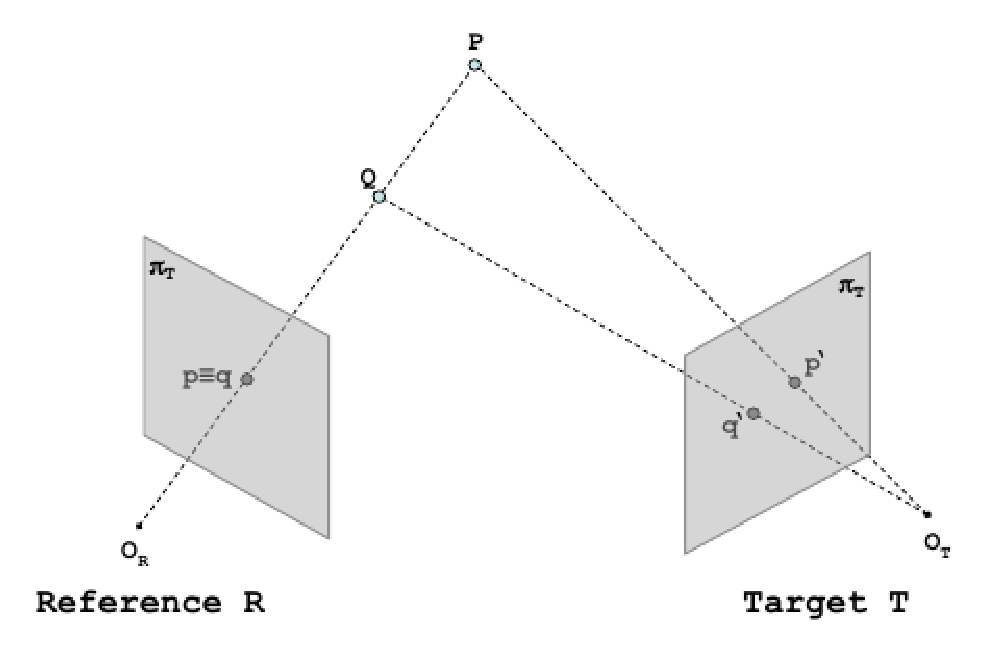
\includegraphics[width=0.7\textwidth]{images/cap2/VisionEstereo.eps}
    \caption{Diferencias entre una y dos cámaras}
    \label{fig:VisionEstereo}
  \end{center}
\end{figure}

Con estos datos, se pueden poner en correspondencia cada punto de ambas
imágenes, para obtener una imagen de disparidad (más información en la sección 
2.2.4).

%--------------------------------------
\subsection{Geometría de las cámaras}
% https://en.wikipedia.org/wiki/Parallax
% http://www.cesfelipesegundo.com/revista/articulos2011/Guerrero,%20J.M.pdf
En función de la posición relativa de las cámaras entre sí, se pueden apreciar
dos métodos principales:

\begin{itemize}
  \item \textbf{Visión paralela:} las cámaras están paralelas entre sí y están
  separadas por una línea horizonal (línea base). El objetivo que visualiza
  cada cámara es perpendicular respecto a la línea base, mientras que las
  líneas de correspondencia que unen los puntos de una imagen respecto a la otra
  son horizontales.

  \begin{minipage}{\linewidth}
      \centering
      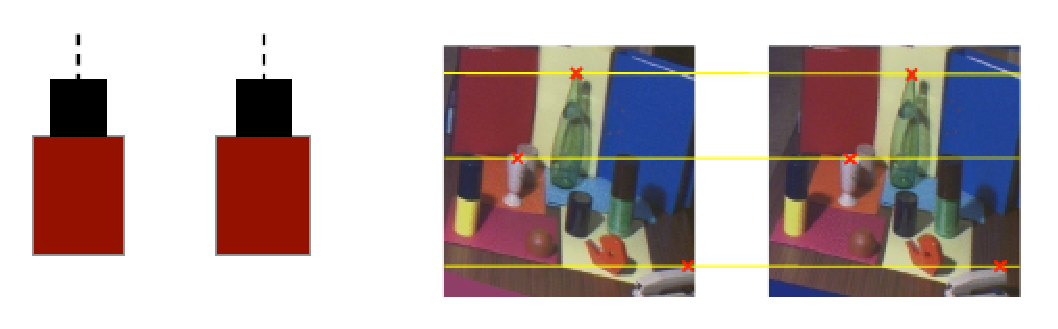
\includegraphics[width=0.7\textwidth]{images/cap2/VisionParalela.eps}
      \captionof{figure}{Visión paralela}
      \label{fig:VisionParalela}
  \end{minipage}

  \item \textbf{Visión cruzada:} las cámaras no están paralelas entre sí, tienen
  una inclinación de tal forma que el objetivo de cada cámara apunta hacia el
  lado contrario de una imagen. Por lo que los ejes ópticos se cruzan entre sí.
  Las líneas de correspondencia, también tienen sufren una inclinación.

  \begin{minipage}{\linewidth}
      \centering
      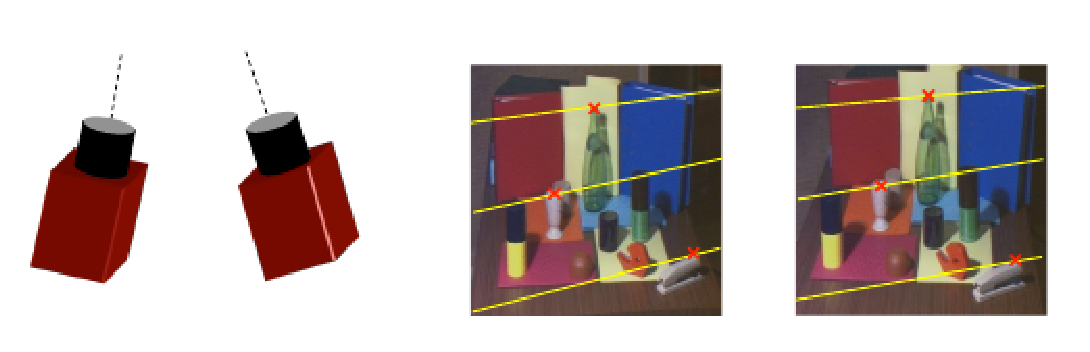
\includegraphics[width=0.7\textwidth]{images/cap2/VisionCruzada.eps}
      \captionof{figure}{Visión cruzada}
      \label{fig:VisionCruzada}
  \end{minipage}
\end{itemize}

% http://vfxio.com/PDFs/Parallel_vs_Converged.pdf
La visión cruzada tiene la desventaja de distorsionar las imágenes capturadas.
En la figura 2.4 se puede observar este efecto al fotografíar un muro de
ladrillos. Sin embargo, dependiendo del tipo de escena que se capture, esta
distorsión puede suponer un problema o no.

\begin{figure}[!th]
  \begin{center}
    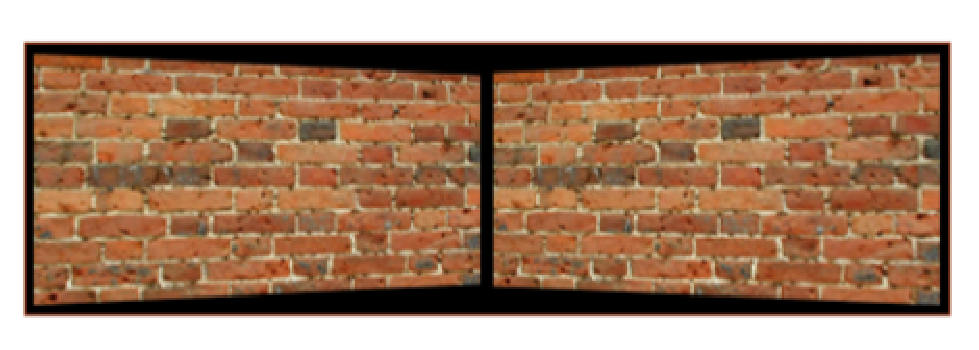
\includegraphics[width=0.5\textwidth]{images/cap2/VisionCruzadaMuro.eps}
    \caption{Muro distorsionado por visión cruzada}
    \label{fig:VisionCruzadaMuro}
  \end{center}
\end{figure}

La visión paralela por su parte, no distorsiona las imágenes capturadas, pero
también cuenta con otra serie de problemas. \textcolor{red}{Lorem ipsum dolor sit amet, consectetur adipisicing elit, sed do eiusmod tempor incididunt ut labore et dolore magna aliqua. Ut enim ad minim veniam, quis nostrud exercitation ullamco laboris nisi ut aliquip ex ea commodo consequat. Duis aute irure dolor in reprehenderit in voluptate velit esse cillum dolore eu fugiat nulla pariatur. Excepteur sint occaecat cupidatat non proident, sunt in culpa qui officia deserunt mollit anim id est laborum.}

%--------------------------------------
\subsection{Rectificación}
% https://en.wikipedia.org/wiki/Image_rectification

%--------------------------------------
\subsection{Disparidad}
% http://es.slideshare.net/RicardoSnchezCastill/vision-artificial-49264591
% http://stackoverflow.com/questions/17607312/difference-between-disparity-map-and-disparity-image-in-stereo-matching
% http://iie.fing.edu.uy/publicaciones/2005/Lec05a/Lec05a.pdf
La disparidad de dos imágenes establece la correspondencia entre los píxeles o
características que existen entre ambas para obtener la profundidad de la
escena. Conociendo la geometría del entorno y la cámara, de forma general, se
realiza una triangulación entre cada punto de las imágenes para obtener la
disparidad.

Metodos:


El objetivo final es poder construir una \textbf{imagen o mapa de disparidad}







% Disparidad....

% http://www.cesfelipesegundo.com/revista/articulos2011/Guerrero,%20J.M.pdf
% http://dmi.uib.es/~abasolo/cursorealidad/paco/Estereoscopia.html
%--------------------------------------
\subsection{Aplicaciones}
% https://www.ptgrey.com/tan/10570
La visión artificial resulta de gran utilidad en diferentes áreas de aplicación,
tanto en acciones repetitivas como peligrosas:

\begin{itemize}
  \item \textbf{Inspección y ensamblaje industrial:} el proyecto "Randon Bin
  Picking" (RBP) hace uso de visión estéreo para la búsqueda de piezas entre
  objetos de todo tipo para su rápida recuperación.
  % http://www.worldscientific.com/doi/suppl/10.1142/8766/suppl_file/8766_chap01.pdf
  \item \textbf{Apoyo en el diagnóstico médico:} en las últimas décadas la
  visión artificial se ha hecho un importante en la medicina para detectar,
  analizar y reconstruir la información obtenida.
  % http://www.ri.cmu.edu/pub_files/pub4/matthies_larry_2007_1/matthies_larry_2007_1.pdf
  \item \textbf{Exploración espacial:} en el proyecto de exploración Mars Rover
  (Mars Exploration Rover Mission) tiene como objetivo explorar la superficie
  de Marte en busca de rocas u otros elementos que prueben la existencia de
  agua.
  \item \textbf{Seguimiento (Tracking):} se hace uso en innumerables situaciones
  de carácter estadístico como contar el número o de en áreas de vigilancia y
  seguridad monitorizando trayectorias.
\end{itemize}


%+++++++++++++++++++++++++++++++++++++++++++++++++++++++++++++++++++++++++++++++
\section{Odometría}
\label{2:sec:3}

%--------------------------------------
\subsection{Mecánica}

%--------------------------------------
\subsection{Visual}


%+++++++++++++++++++++++++++++++++++++++++++++++++++++++++++++++++++++++++++++++
\section{Reconstrucción 3D}
\label{2:sec:4}


% http://slipguru.disi.unige.it/OLDslipguru/teaching/Vis2/LUCIDI/class5.pdf

% nube de puntos


%--------------------------------------
\subsection{SLAM}


%+++++++++++++++++++++++++++++++++++++++++++++++++++++++++++++++++++++++++++++++








